\documentclass[12pt,a4paper]{article}

\setlength{\textwidth}{165mm}
\setlength{\textheight}{240mm}
\setlength{\parindent}{0mm} % S{\aa} meget rykkes ind efter afsnit
\setlength{\parskip}{\parsep}
\setlength{\headheight}{0mm}
\setlength{\headsep}{0mm}
\setlength{\hoffset}{-2.5mm}
\setlength{\voffset}{0mm}
\setlength{\footskip}{15mm}
\setlength{\oddsidemargin}{0mm}
\setlength{\topmargin}{0mm}
\setlength{\evensidemargin}{0mm}

\usepackage[all]{xy}
\usepackage{graphicx}    % For grafik (billederfiler)
\usepackage[T1]{fontenc} % For at blande \textsc{} med \textbf{}
\usepackage[utf8]{inputenc}
\usepackage{amsfonts,amsmath,amssymb}
\usepackage{eucal}
\usepackage[danish]{babel}
\usepackage{enumerate}  
\usepackage{hyperref}
\usepackage{url}
\usepackage{mathptmx}
\usepackage{multirow}
\usepackage[dvipsnames,usenames]{color}
\usepackage{tabularx,colortbl,xcolor}
\usepackage{listings}
\usepackage{color}
\usepackage{amsmath}
\usepackage{xcolor}

\definecolor{KU-red}{RGB}{144,26,30} 
\definecolor{dkgreen}{rgb}{0,0.6,0}
\definecolor{gray}{rgb}{0.5,0.5,0.5}
\definecolor{mauve}{rgb}{0.58,0,0.82}

\lstset{frame=tb,
  language=Java,
  aboveskip=3mm,
  belowskip=3mm,
  showstringspaces=false,
  columns=flexible,
  basicstyle={\small\ttfamily},
  numbers=none,
  numberstyle=\tiny\color{gray},
  keywordstyle=\color{blue},
  commentstyle=\color{dkgreen},
  stringstyle=\color{mauve},
  breaklines=true,
  breakatwhitespace=true,
  tabsize=3}

\DeclareSymbolFont{usualmathcal}{OMS}{cmsy}{m}{n}
\DeclareSymbolFontAlphabet{\mathcal}{usualmathcal}
\DeclareSymbolFont{letters}{OML}{txmi}{m}{it}

\DeclareMathSymbol{\alpha}{\mathord}{letters}{"0B}
\DeclareMathSymbol{\beta}{\mathord}{letters}{"0C}
\DeclareMathSymbol{\gamma}{\mathord}{letters}{"0D}
\DeclareMathSymbol{\delta}{\mathord}{letters}{"0E}
\DeclareMathSymbol{\epsilon}{\mathord}{letters}{"0F}
\DeclareMathSymbol{\zeta}{\mathord}{letters}{"10}
\DeclareMathSymbol{\eta}{\mathord}{letters}{"11}
\DeclareMathSymbol{\theta}{\mathord}{letters}{"12}
\DeclareMathSymbol{\iota}{\mathord}{letters}{"13}
\DeclareMathSymbol{\kappa}{\mathord}{letters}{"14}
\DeclareMathSymbol{\lambda}{\mathord}{letters}{"15}
\DeclareMathSymbol{\mu}{\mathord}{letters}{"16}
\DeclareMathSymbol{\nu}{\mathord}{letters}{"17}
\DeclareMathSymbol{\xi}{\mathord}{letters}{"18}
\DeclareMathSymbol{\pi}{\mathord}{letters}{"19}
\DeclareMathSymbol{\rho}{\mathord}{letters}{"1A}
\DeclareMathSymbol{\sigma}{\mathord}{letters}{"1B}
\DeclareMathSymbol{\tau}{\mathord}{letters}{"1C}
\DeclareMathSymbol{\upsilon}{\mathord}{letters}{"1D}
\DeclareMathSymbol{\phi}{\mathord}{letters}{"1E}
\DeclareMathSymbol{\chi}{\mathord}{letters}{"1F}
\DeclareMathSymbol{\psi}{\mathord}{letters}{"20}
\DeclareMathSymbol{\omega}{\mathord}{letters}{"21}
\DeclareMathSymbol{\varepsilon}{\mathord}{letters}{"22}
\DeclareMathSymbol{\vartheta}{\mathord}{letters}{"23}
\DeclareMathSymbol{\varpi}{\mathord}{letters}{"24}
\DeclareMathSymbol{\varrho}{\mathord}{letters}{"25}
\DeclareMathSymbol{\varsigma}{\mathord}{letters}{"26}
\DeclareMathSymbol{\varphi}{\mathord}{letters}{"27}
\DeclareMathSymbol{\Gamma}{\mathord}{letters}{"00}
\DeclareMathSymbol{\Delta}{\mathord}{letters}{"01}
\DeclareMathSymbol{\Theta}{\mathord}{letters}{"02}
\DeclareMathSymbol{\Lambda}{\mathord}{letters}{"03}
\DeclareMathSymbol{\Xi}{\mathord}{letters}{"04}
\DeclareMathSymbol{\Pi}{\mathord}{letters}{"05}
\DeclareMathSymbol{\Sigma}{\mathord}{letters}{"06}
\DeclareMathSymbol{\Upsilon}{\mathord}{letters}{"07}
\DeclareMathSymbol{\Phi}{\mathord}{letters}{"08}
\DeclareMathSymbol{\Psi}{\mathord}{letters}{"09}
\DeclareMathSymbol{\Omega}{\mathord}{letters}{"0A}
\DeclareMathSymbol{\upGamma}{\mathalpha}{operators}{"00}
\DeclareMathSymbol{\upDelta}{\mathalpha}{operators}{"01}
\DeclareMathSymbol{\upTheta}{\mathalpha}{operators}{"02}
\DeclareMathSymbol{\upLambda}{\mathalpha}{operators}{"03}
\DeclareMathSymbol{\upXi}{\mathalpha}{operators}{"04}
\DeclareMathSymbol{\upPi}{\mathalpha}{operators}{"05}
\DeclareMathSymbol{\upSigma}{\mathalpha}{operators}{"06}
\DeclareMathSymbol{\upUpsilon}{\mathalpha}{operators}{"07}
\DeclareMathSymbol{\upPhi}{\mathalpha}{operators}{"08}
\DeclareMathSymbol{\upPsi}{\mathalpha}{operators}{"09}
\DeclareMathSymbol{\upOmega}{\mathalpha}{operators}{"0A}

\newcommand{\hhemail}[1]{\textsf{#1}}
\newcommand{\hhurl}[1]{{\color{blue}\url{#1}}}

\begin{document}
	
	\begin{minipage}[b]{1.0\linewidth} 
		
\includegraphics[height=50mm]{KULogo.pdf}
		
		\vspace*{-16ex}
		\vspace {35ex}
		\begin{center}
			{\huge \bf Project: Beetle} \\
			{\huge\textit {Assignments}}\vspace*{4ex} \\
			{\large 23. march 2014}\\
			\vspace*{2ex}
			qzj710 - 121095 - Enes Golic \\
			rpc308 - 070493 - Yunus Emre Okutan \\
			cbh239 - 250594 - Casper Lützhøft Christensen \\
			mhb558 - 250795 - Tor-Salve Dalsgaard\\
			\vspace*{1ex}
			Instructor - Casper Passau
			
		\end{center}
	\end{minipage}
	
\newpage

\section{OOSE 1.6}
\begin{enumerate}
\item Functional requirement. Enabling a traveller to buy weekly passes is a direct specification of the program’s functionality.
\item Non-functional requirement. That the program must be written in Java has nothing to do with the actual functioning of the program.
\item Non-functional requirement. The program being easy to use is not a specification of a required function in the program.
\item Non-functional requirement. The program’s availability is not a specification of the program’s functioning.
\item Functional requirement. Providing a phone number in case of failure is a direct functional aspect of the program.	
\end{enumerate}

\section{OOSE 1.8}
The usage of account in the context of providing access to an account when the system cannot establish an internet-connection is an application domain concept. This is because it clearly describes a feature desired for the application in question.\\
The usage of account in the context of providing access, even when the server cannot be reached, and simply having the last session displayed is a solution domain concept. The reason is that it is a solution given in order to give the program the desired functionality.

\newpage

\section{OOSE 2.6, 2.7, 2.9 and 2.10}
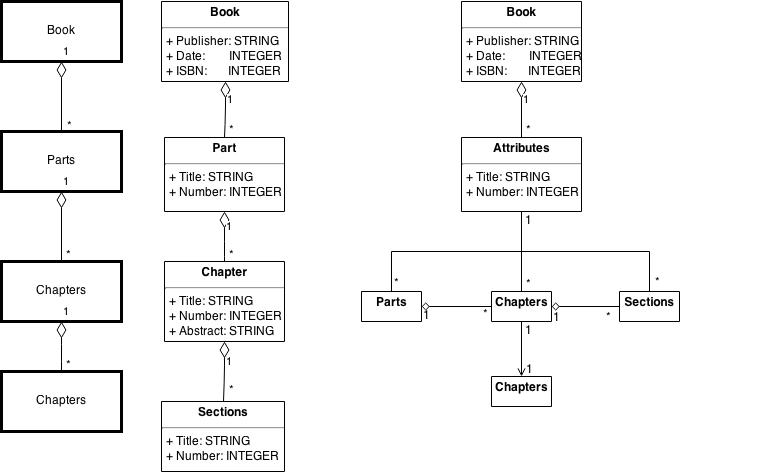
\includegraphics[height=350px]{UntitledDiagram.jpg}

\newpage

\section{OOSE 5.3}
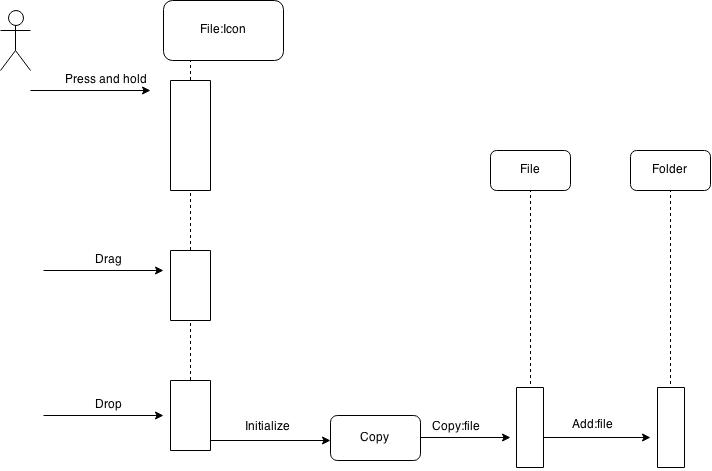
\includegraphics[height=300px]{Sequence.jpg}\\
A USER can click on a specific file and hold, to drag the file and drop it anywhere on the screen. This will initialise the copying of the file in which the new file is then added to a specific folder.

\newpage

\section{OOSE 7.1}
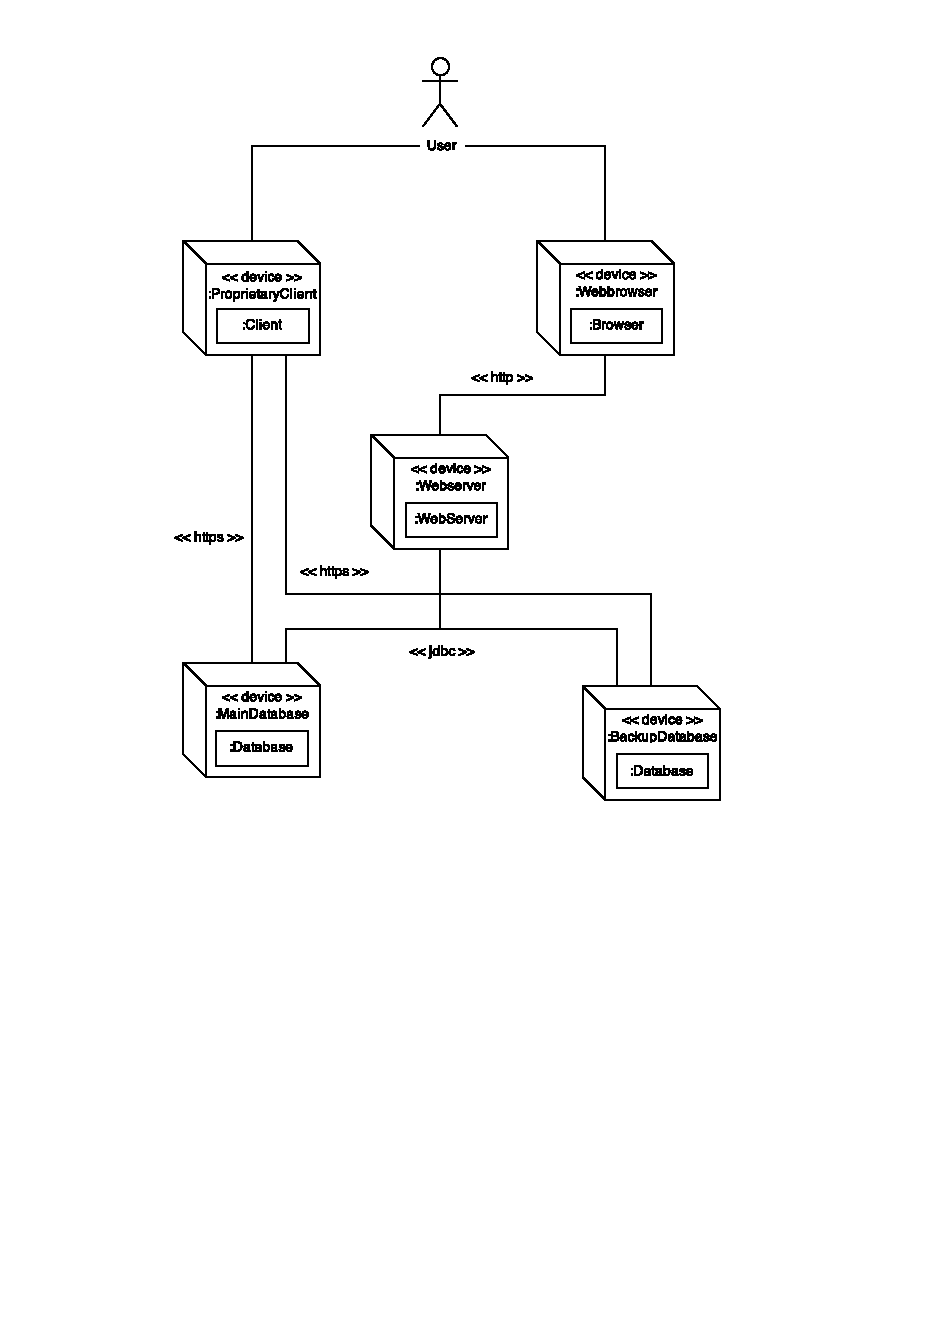
\includegraphics{DeploymentDiagram.pdf}
\end{document}